\documentclass[a4paper, 11pt]{article}
%\usepackage[utf8]{inputenc}
\usepackage{appendix}
\usepackage{listings}
\usepackage{color}
\usepackage{xcolor}
\usepackage{float}
\usepackage[british]{babel}
\usepackage{amsmath}
\usepackage{amsfonts}
\usepackage{amssymb}
\usepackage{amsthm}
%\usepackage{amsrefs}
\usepackage{enumerate}
\usepackage{graphicx}
\usepackage{caption}
\usepackage{subcaption}
\usepackage{url}
\usepackage[round]{natbib}
\usepackage[all]{xy}
\usepackage{tikz}
\usepackage{hyperref}
\usepackage[percent]{overpic}
\usepackage[printwatermark]{xwatermark}
\usepackage{epstopdf}
\usepackage{fancyvrb}
\usepackage{longtable}
\usepackage{wasysym}
%\usepackage{multicol}
\usepackage{pgfplots}
%\usepackage{newtxtext,newtxmath}
%\newwatermark[allpages,color=red!20,angle=45,scale=4,xpos=0,ypos=0]{DRAFT}

%\usepackage{antpolt}
%\usepackage[T1]{fontenc}
%\usepackage{tocloft}
\usepackage{selinput}
\SelectInputMappings{
  adieresis={ä},
  edieresis={ë},
  idieresis={ï},
  udieresis={ü},
  eacute={é},
}

\newcommand{\widefigwidth}{\textwidth}
\newcommand{\mgraphheight}{.21\textheight}

\usetikzlibrary{positioning}

\definecolor{MidnightBlue}{RGB}{11,28,121}
\definecolor{dkgreen}{rgb}{0,0.6,0}
\definecolor{mauve}{rgb}{0.58,0,0.82}

\newcommand{\citeneed}{{\color{red} [citation needed] }}
\newcommand{\citepos}{{\color{orange} [citation needed?] }}
\newcommand{\todo}[1]{{\color{red} TODO:} {\color{dkgreen} #1}}
\newcommand{\ennl}[1]{{\color{red} \it [TL: #1]}}

\newcommand{\Python}{\texttt{Python}}

\renewcommand{\thefigure}{\arabic{section}.\arabic{figure}}

\newcommand{\mat}[1]{\left(\begin{matrix} #1 \end{matrix} \right)}
\newcommand{\HRule}{\rule{\linewidth}{0.5mm}}
%\renewcommand{\cftdot}{}
%\renewcommand{\cftsecleader}{\cftdotfill{\cftdotsep}}
\setcounter{tocdepth}{3}

\usepackage{tikz}
\usetikzlibrary{shapes,arrows}

\floatstyle{ruled}
\newfloat{example}{htb}{lop}
\floatname{example}{Example}
\newfloat{codeblok}{htb}{lop}
\floatname{codeblok}{Codeblok}

%\newcommand{\citep}[1]{\cite{#1}}\newcommand{\citet}[1]{\cite{#1}}
\renewcommand{\cite}[1]{\citep{#1}}

\renewcommand{\lstlistingname}{Codeblok}
\lstdefinestyle{lstjava}{
language=Java,
numbers=left,
numberstyle=\tiny\color{red},
stepnumber=5,
numbersep=5pt,
tabsize=2,
breaklines=true,
keywordstyle=\color{MidnightBlue},
commentstyle=\color{dkgreen},
stringstyle=\color{mauve},
morekeywords={}
}
\lstdefinestyle{lstmatlab}{
language=Matlab,
numbers=left,
numberstyle=\tiny\color{red},
stepnumber=5,
numbersep=5pt,
tabsize=2,
breaklines=true,
keywordstyle=\color{MidnightBlue},
commentstyle=\color{dkgreen},
stringstyle=\color{mauve},
morekeywords={linreg,linregquad,logreg,ones,repmat}
}
\lstnewenvironment{lstmat}{
\lstset{style=lstmatlab}}{}

\lstnewenvironment{lstsource}{
\lstset{
language=C,
breaklines=true,
showspaces=false,
showstringspaces=false,
showtabs=false,
morekeywords={}
}}{}

\lstdefinestyle{lstcpp}{
language=C++,
numbers=left,
numberstyle=\tiny\color{red},
stepnumber=5,
numbersep=5pt,
tabsize=2,
breaklines=true,
keywordstyle=\color{MidnightBlue},
commentstyle=\color{dkgreen},
stringstyle=\color{mauve},
morekeywords={}
}


\title{Automatic Plastic Soup Solver\\ {\Large Literature draft}}
\author{student: \\Ysbrand Galama \\ 10262067 \and supervisor: \\ Thomas Mensink}
\date{\today}

\begin{document}
\maketitle

\section*{Problem definition} Large amounts of plastic waste end up in the world's oceans and have a big impact on the marine life \citep{barnes2005drifting}.
A collective noun for this environmental problem is Plastic Soup or Plastic Ocean.
Because the plastic does not decay in nature, a lot of marine life gets the plastic in their digestive system.

Several organisations are working on solving this environmental hazard.
One of them is Saraswater.
They are developing ships that shovel the plastic from the water.
The proposed thesis project could help to automate that process.
If an autonomous agent could detect from cameras where the plastic is, the ships could be controlled by this agent to clean it up.

This project would start the development of this autonomous agent by giving it ``eyes''. The main question is how the current state-of-the-art techniques in image recognition could be used to detect floating plastic in the ocean.

To accomplice the plastic detection in images, the usage of a trained Convolutial Neural Network (CNN) will be tested. The baseline of this test will determine if the plastic recognition will also be used on segmented images, which are not annotated. If the baseline is not adequate, other imagery-techniques will be tested. These techniques will include texture recognition and SIFT with the usage of fisher vectors. In addition the necessarily of colour will be tested.

\section*{CMap}
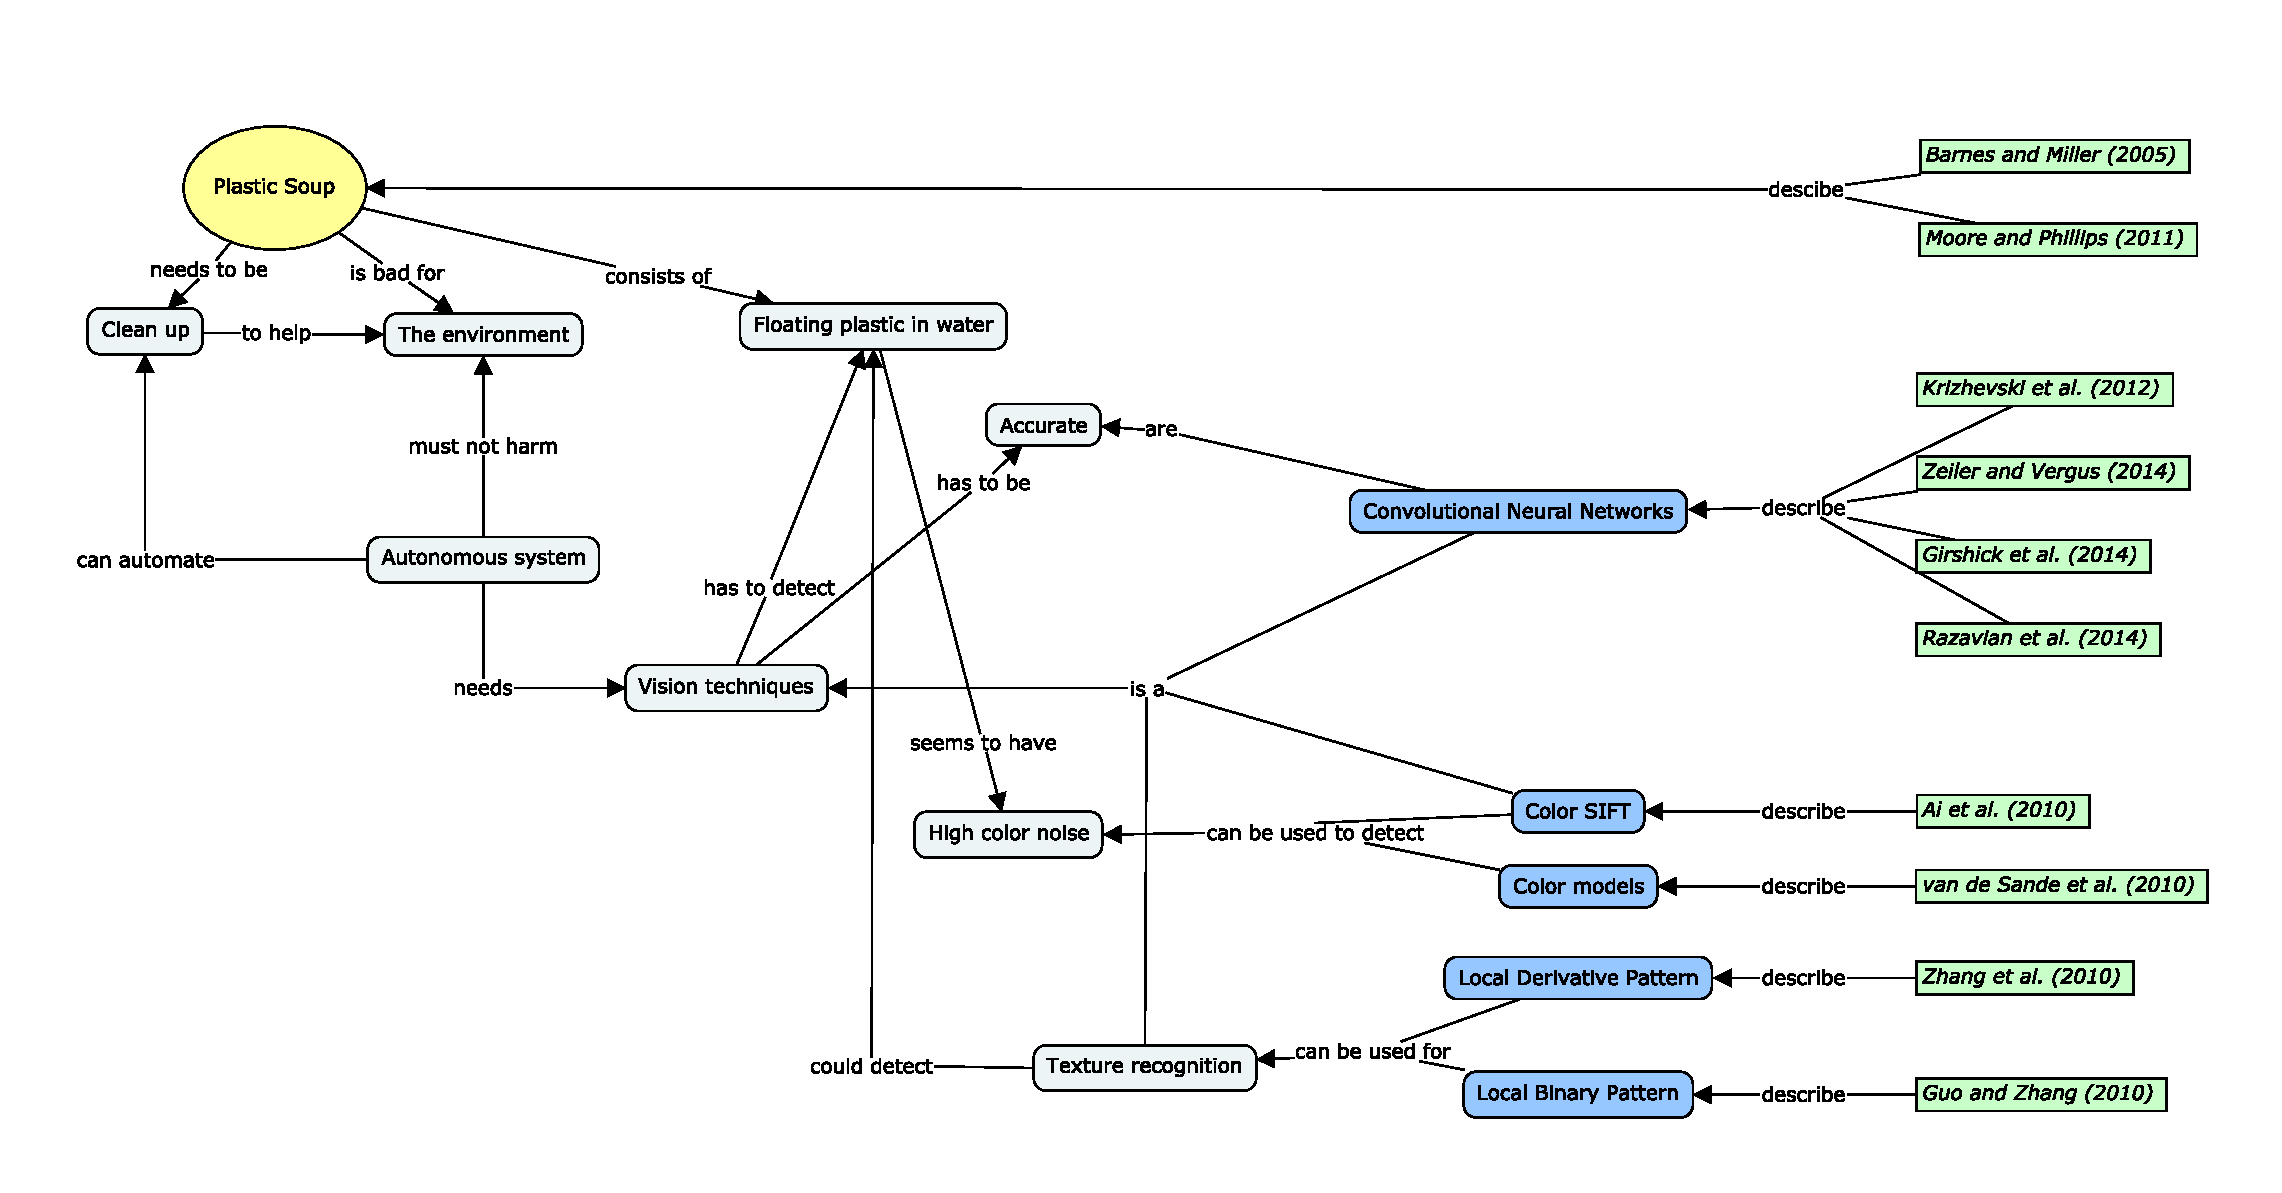
\includegraphics[width=\textwidth]{images/scriptie_1.pdf}

\section*{Literature}
\paragraph{Plastic Soup} To indicate the environmental hazard of the Plastic Soup, two papers will be used, namely \citet{barnes2005drifting} and \citet{moore2011plastic}. In addition several news paper articles can be used to show the public awareness.

\paragraph{Convolutional Neural Networks} The state-of-the-art technique that will be used in this project comes from \citet{krizhevsky2012imagenet}. To understand the CNN better, \citet{zeiler2014visualizing} will help.
Moreover, \citet{girshick2014rich} and \citet{razavian2014cnn} show that applying a CNN is a promising baseline to start.

\paragraph{Textures} Besides the CNN, this project will also research the diferent texture recognition techniques and their application on the Plastic Soup image data. Local binary patterns \citep{guo2010completed} and local derivative patterns \citep{zhang2010local} will be used in this case. Probably a combination of a CNN with these techniques will be used.

\paragraph{Other imagery techniques} On the usage of fisher vectors, \citet{sanchez2013image} is a place to start. The colour model of \citet{van2010evaluating} will be used, as will the possibilities of Colour SIFT \citep{ai2010color}

\vfill
\bibliographystyle{abbrvnat}
\bibliography{Tex_sources/bib}
\end{document}